\documentclass[11pt,oneside,letterpaper]{article}

% graphicx package, useful for including eps and pdf graphics
\usepackage{graphicx}
\DeclareGraphicsExtensions{.pdf,.png,.jpg}

% basic packages
\usepackage{color}
\usepackage{parskip}
\usepackage{float}

% text layout
\usepackage{geometry}
\geometry{textwidth=15cm} % 15.25cm for single-space, 16.25cm for double-space
\geometry{textheight=22cm} % 22cm for single-space, 22.5cm for double-space

% helps to keep figures from being orphaned on a page by themselves
\renewcommand{\topfraction}{0.85}
\renewcommand{\textfraction}{0.1}

% bold the 'Figure #' in the caption and separate it with a period
% Captions will be left justified
\usepackage[labelfont=bf,labelsep=period,font=small]{caption}

% review layout with double-spacing
%\usepackage{setspace}
%\doublespacing
%\captionsetup{labelfont=bf,labelsep=period,font=doublespacing}

% cite package, to clean up citations in the main text. Do not remove.
\usepackage{cite}
%\renewcommand\citeleft{(}
%\renewcommand\citeright{)}
%\renewcommand\citeform[1]{\textsl{#1}}

% Remove brackets from numbering in list of References
\renewcommand\refname{\large References}
\makeatletter
\renewcommand{\@biblabel}[1]{\quad#1.}
\makeatother

\usepackage{authblk}
\renewcommand\Authands{ \& }
\renewcommand\Authfont{\normalsize \bf}
\renewcommand\Affilfont{\small \normalfont}
\makeatletter
\renewcommand\AB@affilsepx{, \protect\Affilfont}
\makeatother

% notation
\usepackage{amsmath}
\usepackage{amssymb}

% Inline comments by initials
\def\jhc#1{\textcolor{red}{[#1]}}
\definecolor{purple}{rgb}{0.459,0.109,0.538}
\def\tbc#1{\textcolor{purple}{[#1]}}
\definecolor{pink}{rgb}{0.8,0.5,0.5}
\def\mfc#1{\textcolor{pink}{[#1]}}

%%% TITLE %%%
\title{\vspace{1.0cm} \Large \bf
Fitness models provide accurate short-term forecasts of SARS-CoV-2 variant frequency
}
%
\author[1,2,*]{Eslam Abousamra}
\author[1,3,*]{Marlin Figgins}
\author[1,2,4]{Trevor Bedford}

\affil[1]{Vaccine and Infectious Disease Division, Fred Hutchinson Cancer Center, Seattle, WA, USA}
\affil[2]{Department of Epidemiology, University of Washington, Seattle, WA, USA}
\affil[3]{Department of Applied Mathematics, University of Washington, Seattle, WA, USA}
\affil[4]{Howard Hughes Medical Institute, Seattle, WA, USA}
\affil[*]{These authors contributed equally to this work.}


\date{}

\begin{document}

\maketitle

%%% ABSTRACT %%%
\begin{abstract}

Genomic surveillance of pathogen evolution is essential for public health response, treatment strategies, and vaccine development.
In the context of SARS-COV-2, multiple models have been developed including Multinomial Logistic Regression (MLR), Fixed Growth Advantage (FGA), Growth Advantage Random Walk (GARW) and Piantham that use observed variant sequence counts through time to analyze variant dynamics.
These models provide estimates of variant fitness and can be used to forecast changes in variant frequency.
We introduce a framework for evaluating real-time forecasts of variant frequencies, and apply this framework to the evolution of SARS-CoV-2 during 2022 in which multiple new viral variants emerged and rapidly spread through the population.
We compare models across representative countries with different intensities of genomic surveillance.
Retrospective assessment of model accuracy highlights that most models of variant frequency perform well and are able to produce reasonable forecasts.
We find that the simple MLR model provides less than 1\% mean absolute error when forecasting 30 days out for countries with robust genomic surveillence.
We investigate impacts of sequence quantity and quality across countries on forecast accuracy and conduct systematically downsampling to identify that 1000 sequences per week is fully sufficient for accurate short-term forecasts.
We conclude that fitness models represent a useful prognostic tool for short-term evolutionary forecasting.

\end{abstract}

%%% INTRODUCTION %%%
\section*{Introduction}

% Paragraph giving overview of SARS-COV-2 genomic surveillance and spread of variant viruses
The emergence of acute respiratory virus SARS-CoV-2 (COVID-19) and its subsequent circulating variants has had far-reaching implications on global health and worldwide economies \cite{onyeaka2021covid19}.
Due to its rapid evolution, original SARS-CoV-2 strains has been replaced by derived, more selectively advantageous variant lineages \cite{campbell2021increased}.
This dynamic landscape has led to emergence of Omicron, a highly transmissible variant that rapidly became the dominant strain altering the spread of COVID-19 \cite{who2022omicron}.
It has become increasingly evident that monitoring the evolution and dissemination of these variants remains crucial with SARS-CoV-2 continuing to evolve beyond Omicron \cite{carabelli2023sarscov2}.
Forecasting variant dynamics allows us to make informed decisions about vaccines and to predict variant-driven epidemics.


% Paragraph giving overview of previous application of fitness models (flu and SARS-CoV-2)
Fitness models are a key resource for forecasting changes in variant frequency or strain frequency through time.
These models were first introduced for the study of seasonal influenza virus \cite{luksza2014predictive, morris2018predictive, huddleston2020integrating} and there have relied on correlates of viral fitness such as mutations to epitope sites on influenza's surface proteins.
In modeling emergence and spread of SARS-CoV-2 variant viruses, the use of Multinomial Logistic Regression (MLR) has become commonplace \cite{annavajhala2021emergence, faria2021genomics, obermeyer2022analysis}.
Here, MLR is analogous to a population genetics model of haploid population in which different variants have a fixed growth advantage and are undergoing Malthusian growth.
As such, it presents a natural model for describing evolution and spread of SARS-CoV-2 variants.
Additionally, models introduced by Figgins and Bedford \cite{figgins2022sars} and by Piantham et al \cite{piantham2021estimating} incorporate case counts and variant-specific Rt, but still can be used to project variant frequencies.

% Broad overview of approach
Here, we systematically assess the predictive accuracy of fitness models for nowcasts and short-term forecasts of SARS-CoV-2 variant frequencies.
We focus on variant dynamics during 2022 in which multiple sub-lineages of Omicron including BA.2, BA.5 and BQ.1 spread rapidly throughout the world.
We compare across several countries including Australia, Brazil, Japan, South Africa, the United Kingdom, and the United States to assess genomic surveillance systems with different levels of throughput and timeliness.
To assess the performance of these models, we used mean and median absolute error (AE) as a metric to compare the predicted frequencies to retrospective truth.
This metric allowed us to evaluate the accuracy and reliability of the models and to identify those that were most effective in predicting SARS-CoV-2 circulating variants trends.
We also examined a variety of variables that contribute to errors in these models and explored the role of sequence availability on nowcast and forecast errors through downsampling sequencing efforts for a sample location.

%%% RESULTS %%%
\section*{Results}

\subsection*{Reconstructing real-time forecasts}

We focus on SARS-CoV-2 sequence data shared to the GISAID EpiCoV database \cite{shu2017gisaid}.
Each sequence is annotated with both a collection date (relevant for understanding dynamics) as well as a submission date.
Here we seek to reconstruct datasets that were actually available on particular dates, and so we use use submission date to filter to sequences that were available at a specific analysis date.
We additionally filter to sequences collected up to 90 days before the analysis date.
We categorize each sequence by Nextstrain clade (21K, 21L, etc\dots) as such clades are generally at a reasonable level of granularity for understanding adaptive dynamics \cite{bloom2023fitness}; there are 7 clades circulating during 2022 vs hundreds of Pango lineages.
Resulting datasets for representative countries Japan and the USA for analysis dates of Apr 1 2022, Jun 1 2022, Sep 1 2022 and Dec 1 2022 are shown in Figure \ref{fig:dynamic_forecast_env}A.
We see consequential backfill in which genome sequences are not immediately available and instead available after a delay due to the necessary bottlenecks of sample acquisition, testing, sequencing, assembly and data deposition.
Thus, even estimating variant frequencies on the analysis date as a nowcast requires extrapolating from past week's data.
Different countries with different genomic surveillance systems have different levels of throughput as well as different amounts of delay between sample collection and sequence submission \cite{brito2022global}.

%%% dynamic_forecast_env %%%
\begin{figure}[tb!]
	\centering
	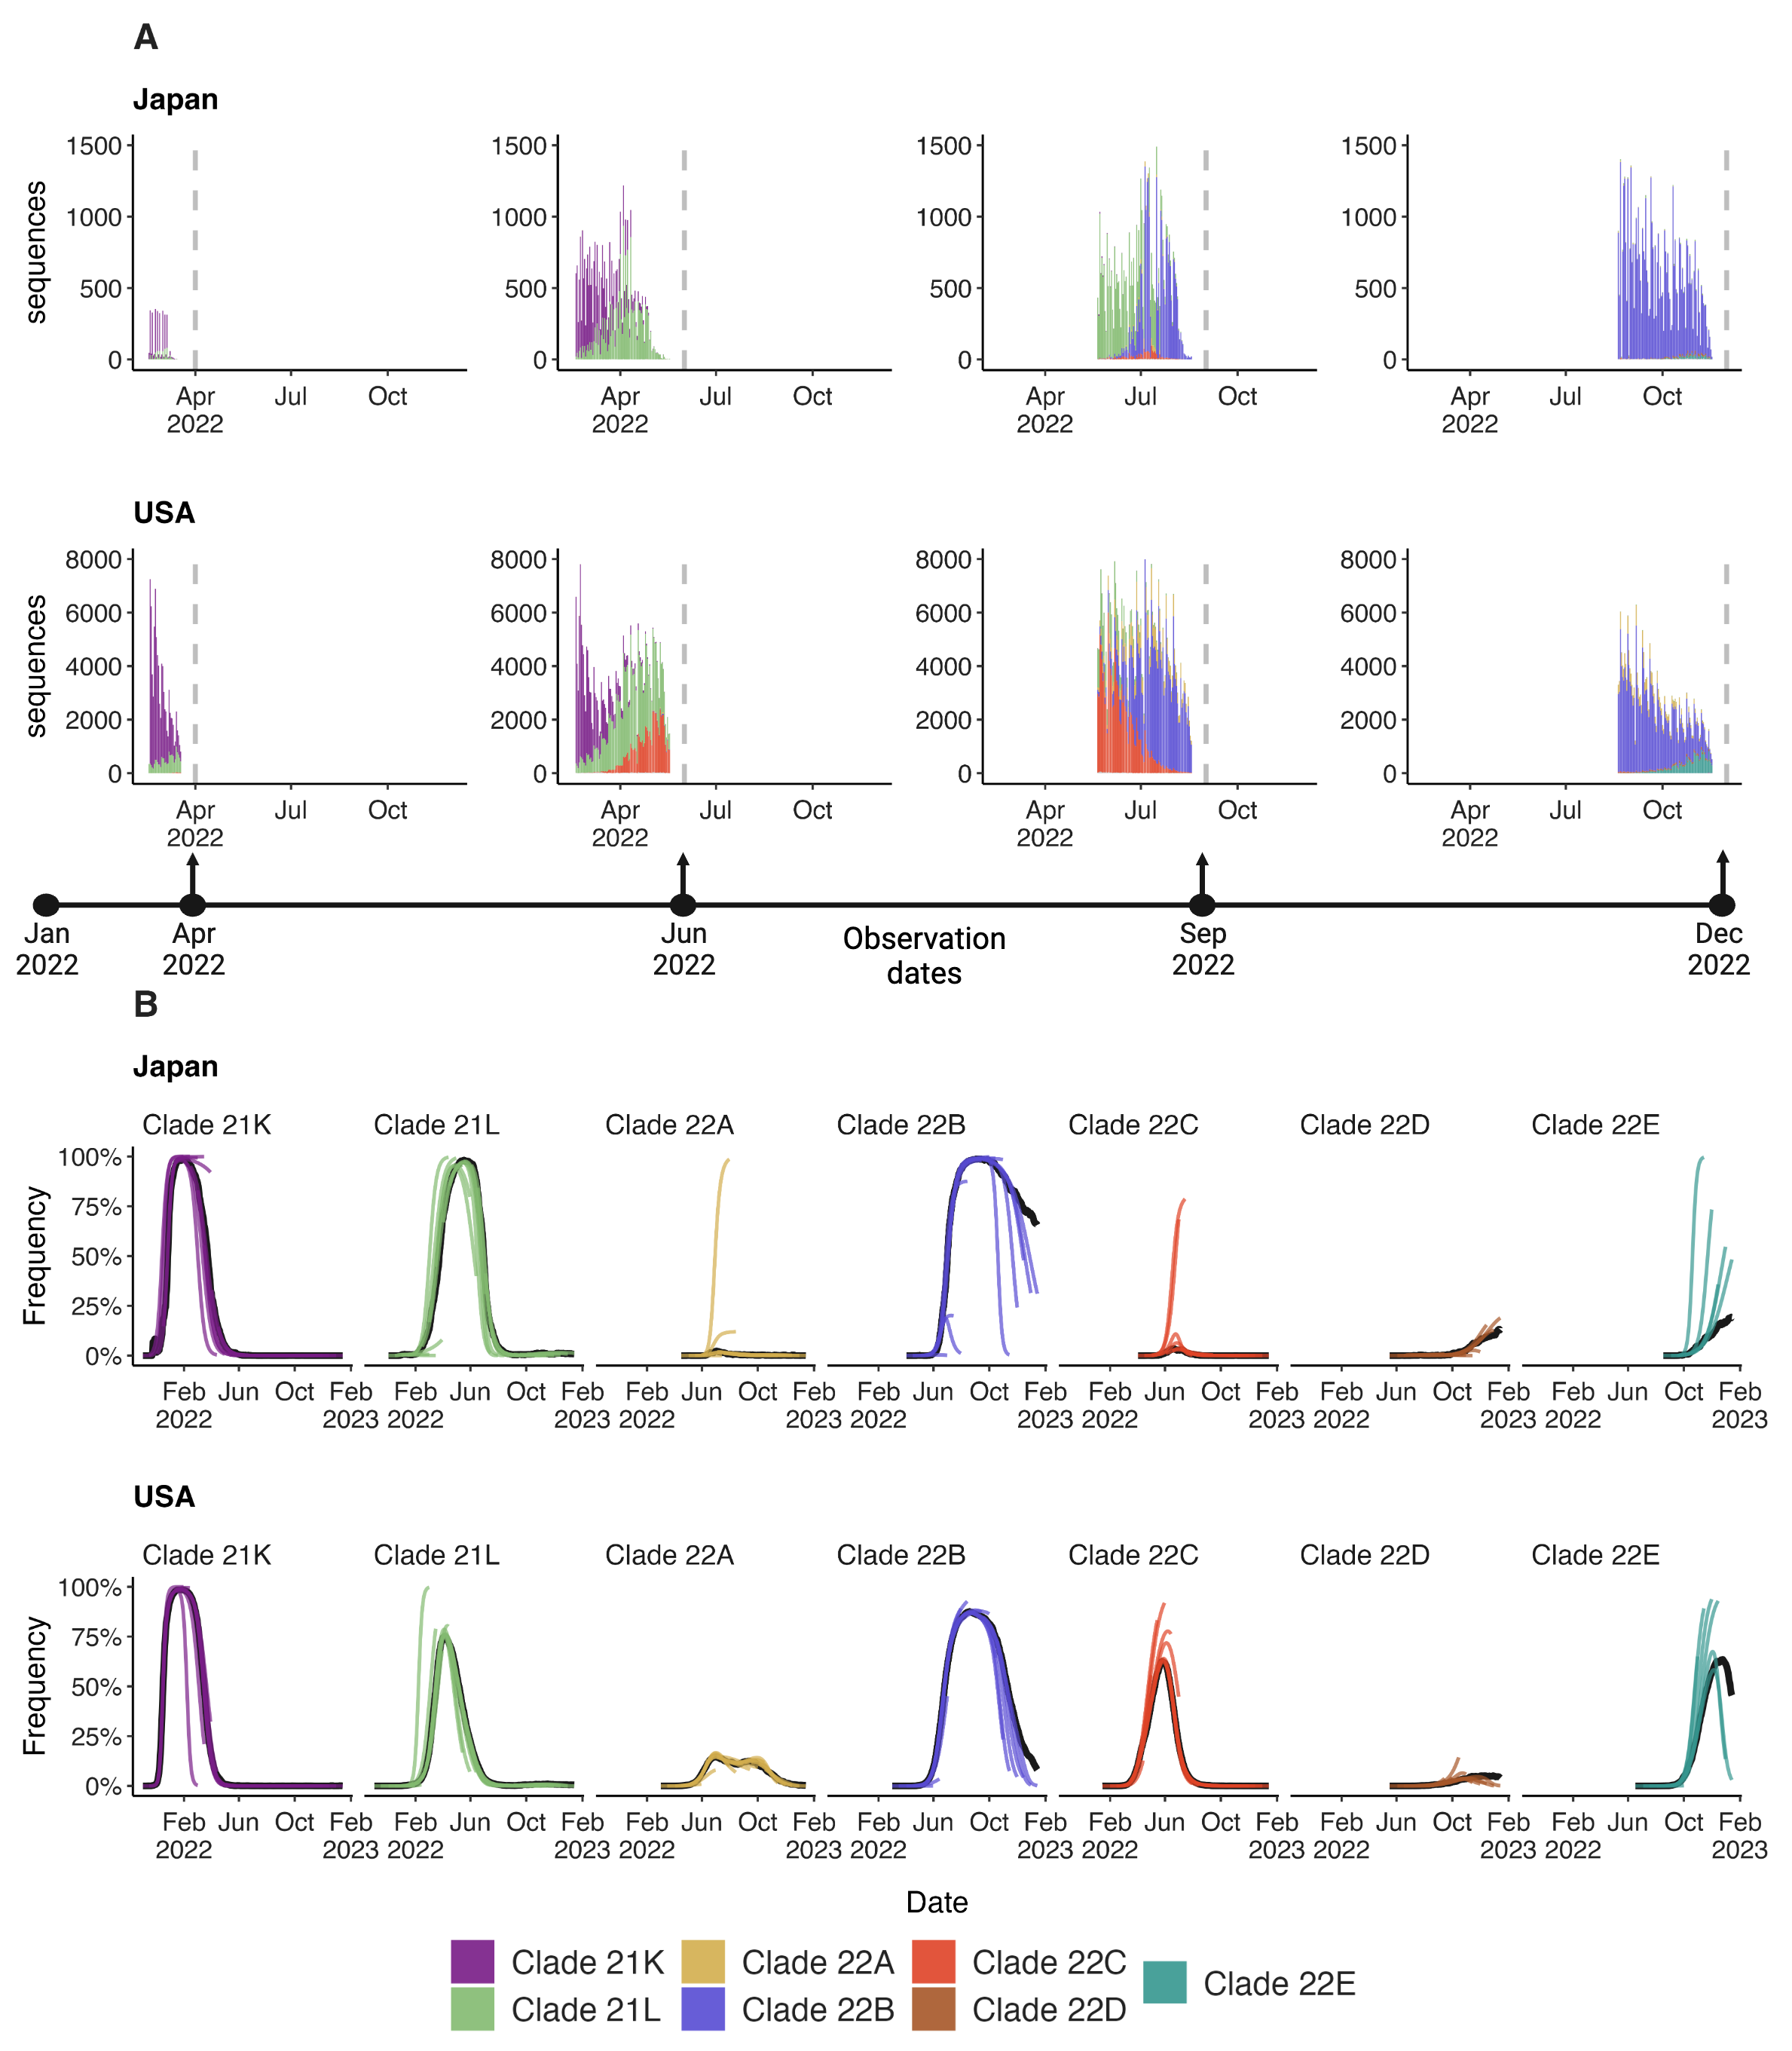
\includegraphics[width=0.9\textwidth=0.01]{figures/Dynamic_est_env.png}
	\caption{
		\textbf{Reconstructing available datasets and corresponding predictions for Japan and USA.}
		(A) Variant sequence counts categorized by Nextstrain clade from Japan and United States at 3 different analysis dates.
		Notice varying sequence availability at different observation dates.
		(B) +30 day frequency forecasts for variants in bimonthly intervals using the GARW variant Rt model.
		Each forecast trajectory is shown as a different colored line.
		Retrospective smoothed frequency is shown as a thick black line.
	}
	\label{fig:dynamic_forecast_env}
\end{figure}

We employ a sliding window in which we conduct an analysis twice each month (on the 1st and the 15th) and estimate variant frequencies from -90 days to +30 days relative to each analysis date.
For this projection we use the variant Rt model \cite{figgins2022sars} parameterized as a Growth Advantage Random Walk (GARW) to estimate variant-specific Rt and and from this changes in variant frequency through time.
Figure \ref{fig:dynamic_forecast_env}B shows resulting trajectories as colored lines.
Sometimes we see initial over-shoot or under-shoot as variant growth and decline, but there is general consistency across trajectories.
\mfc{We should expand of this more. This to me is the main point of interest.}
Additionally, we retrospectively reconstructed the simple 7-day smoothed frequency for across variants and present these trajectories as solid black lines.
We treat this retrospective trajectory as `truth' and thus deviations from model projections and retrospective truth can be assessed to determine nowcast and short-term forecasting accuracy.
Consistent with less available data, we observe that the model predictions for Japan were more frequently misestimated compared to the United States with particularly large differences for clades 22B (lineage BA.5) and 22E (lineage BQ.1) (Fig.~\ref{fig:dynamic_forecast_env}B).

\subsection*{Model error comparison}

\begin{figure}[tb!]
	\centering
	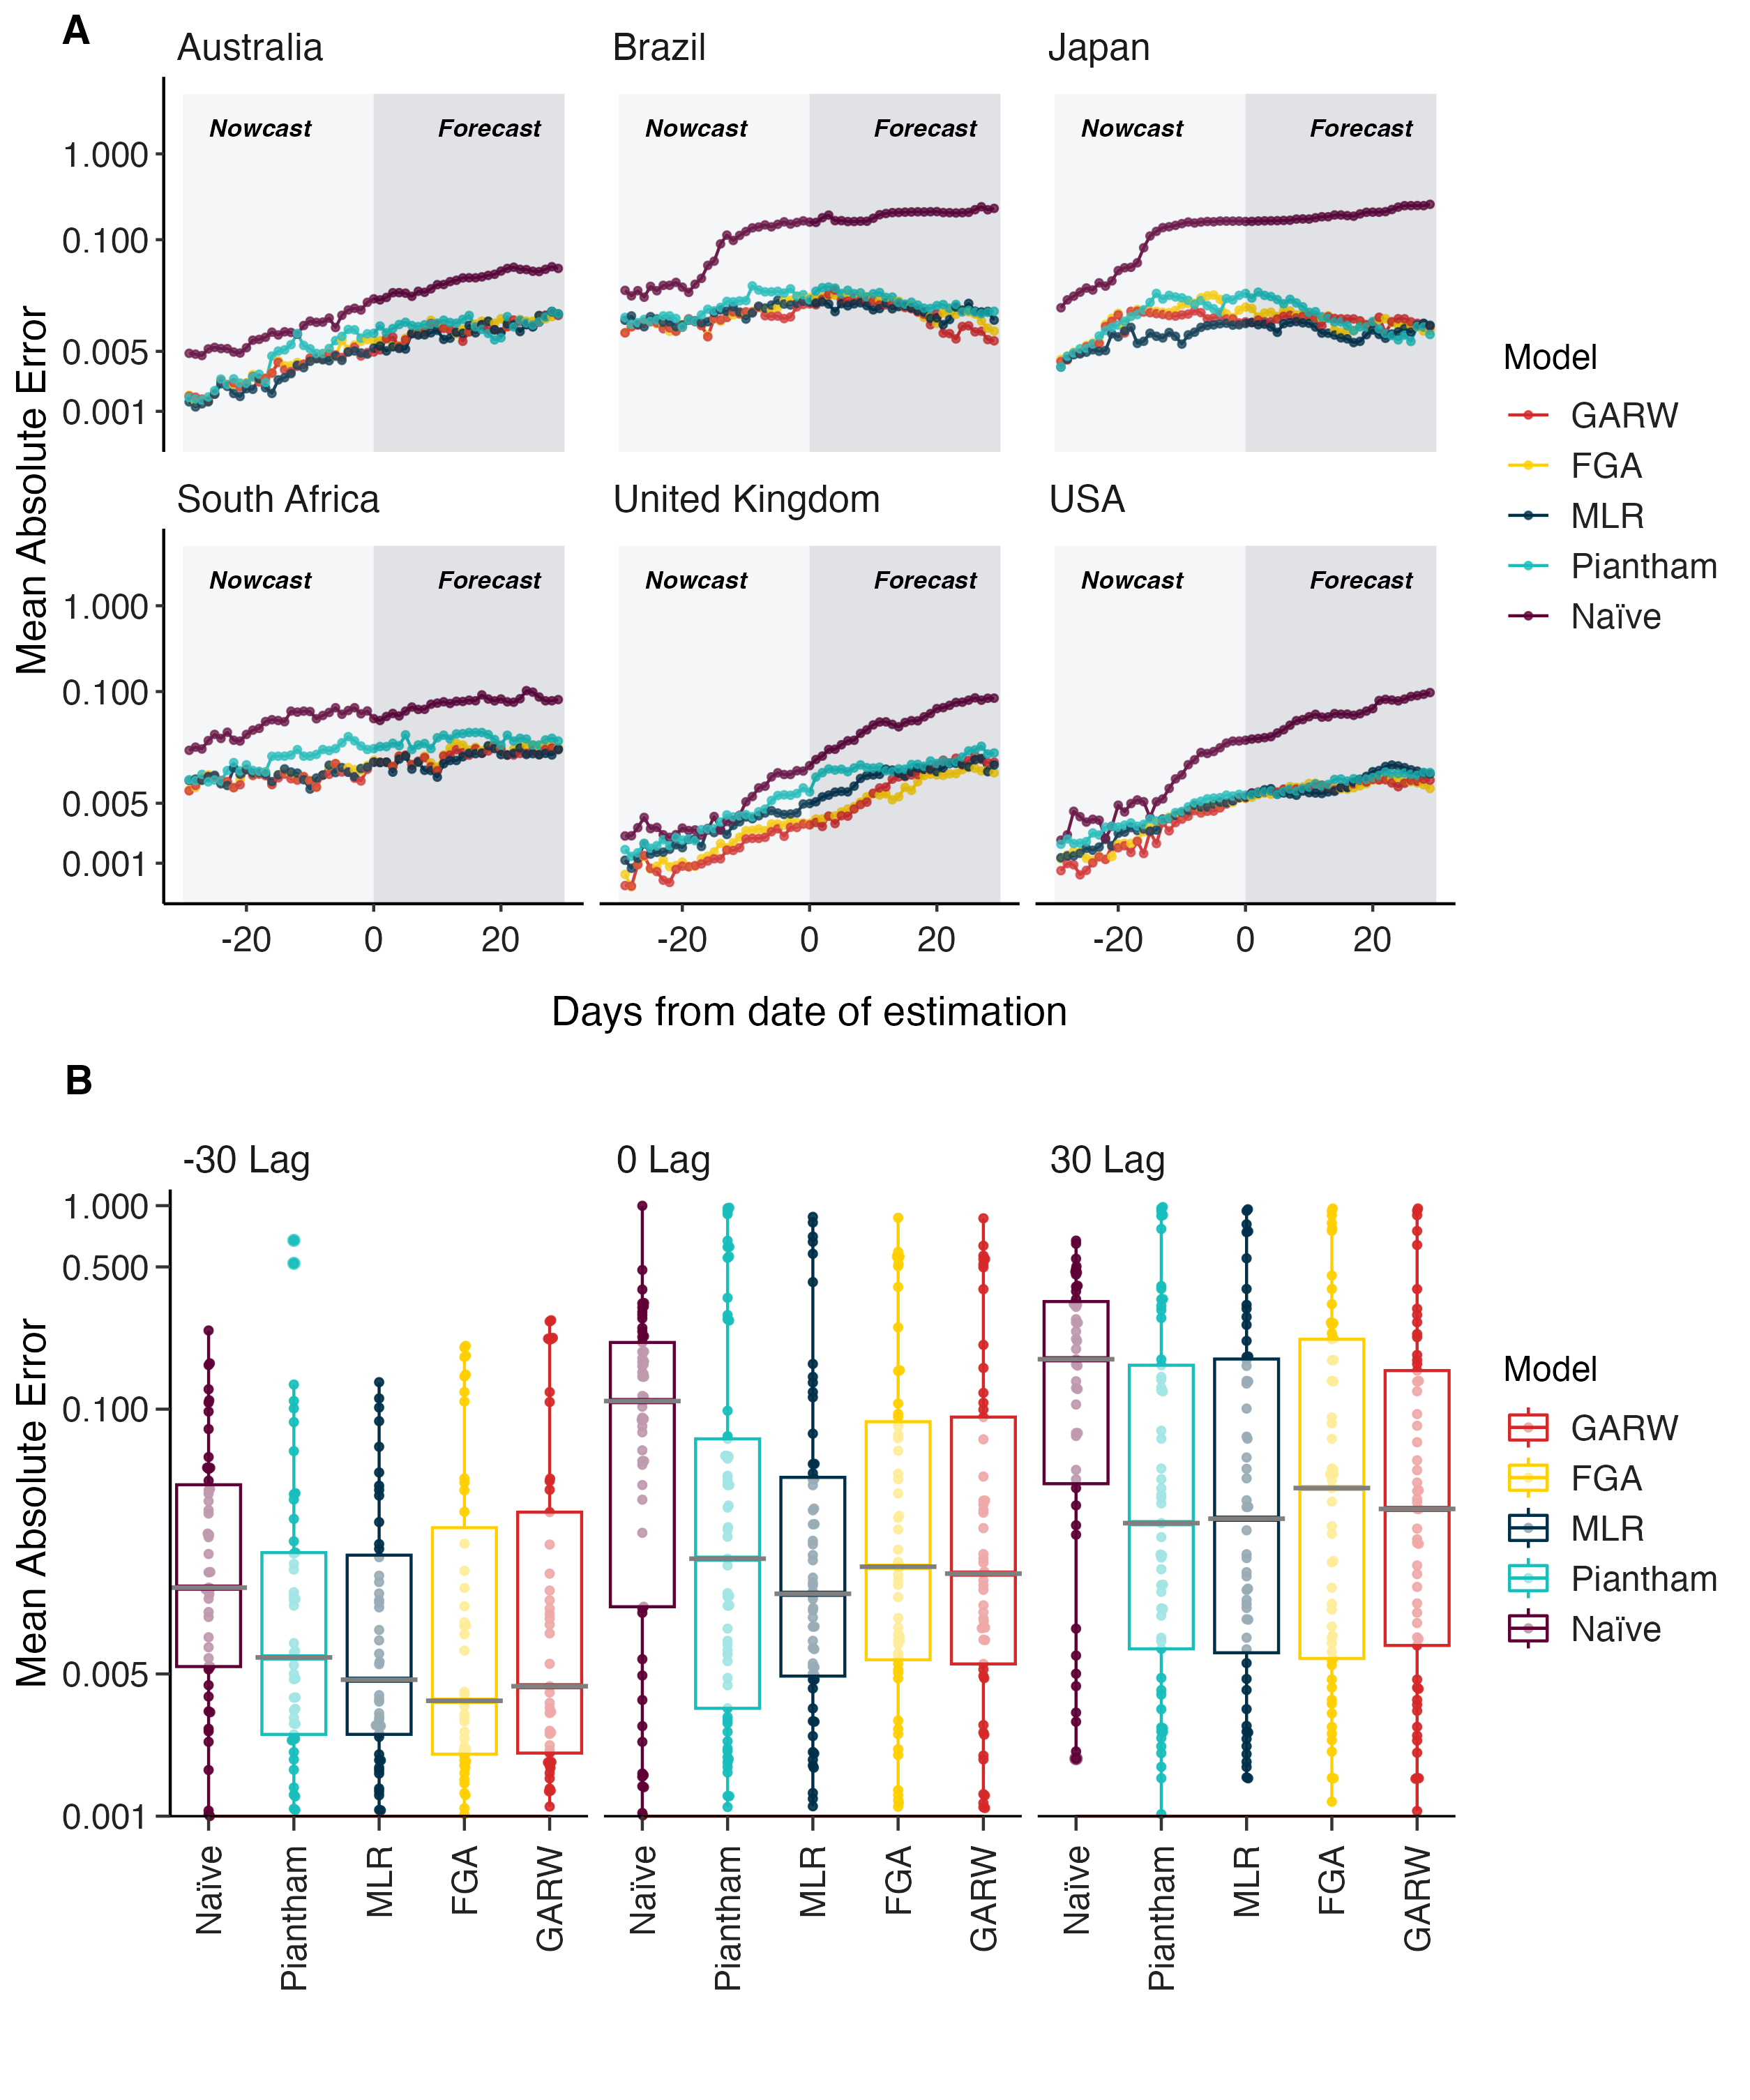
\includegraphics[width=0.9\textwidth]{figures/model_comp.png}
	\caption{\textbf{Absolute error estimates across models and countries.}
	(A) Error increases as forecast target moves from hindcasting at -30 days to nowcasting at 0 days to forecasting at +30 days.
	(B) Distribution of absolute error on a log scale across models and across forecasting lags.
	This shows that most predictions have little error, while a small subset of predictions have large error.
	}
	\label{fig:model_comp_fig}
\end{figure}



We utilize five models for predicting the frequencies of SARS-CoV-2 variants in six countries (Australia, Brazil, Japan, South Africa, the United Kingdom, and the United States).
The simplest of these models is Multinomial Logistic Regression (MLR) commonly used in SARS-CoV-2 analyses \cite{annavajhala2021emergence, faria2021genomics, obermeyer2022analysis}, which uses only clade-specific sequence counts and has a fixed growth advantage for each variant.
More complex models include the Fixed Growth Advantage (FGA) and Growth Advantage Random Walk (GARW) parameterizations of the variant Rt model introduced by Figgins and Bedford \cite{figgins2022sars}, which uses case counts in addition to clade-specific sequence counts.
The Piantham et al model \cite{piantham2021estimating} operates on a similar principle in estimating variant-specific Rt, but differs in model details.
We compare these four models to a naive model to serve as a reference model for comparison.
The naive model implemented as a 7-day moving average on the retrospective raw frequencies using the most recent seven days for which sequencing data is available.
The use of multiple models that range in complexity allows for a comprehensive evaluation of the performance and robustness of different forecasting methods.
We compare forecasting accuracy across different time lags from -30 days back from date of analysis to target hindcast date, to +0 days from date of analysis to target nowcast date, to +30 days forward from date of analysis to target forecast date.

% Throughout the following discussion, we refer to `mean absolute error (AE)' for a specific model $m$, a specific dataset $d$ and a specific forecasting lag $l$ and forecast $p$ as the mean absolute difference between predicted frequency and retrospective frequency across variants $v$
% \begin{equation}
% \mathrm{AE}_{m, d, l, v} = \frac{1}{n} \sum_{v \in V} |f_{m, d, l, v} - \hat{f}_{m, d, l, t}|,
% \end{equation}
% where $f$ represents retrospective frequency and $\hat{f}$ represents the prospective predicted frequency.
% We summarize these AE values across different models, different datasets and different lags either via taking mean AE or taking median AE.

%%% model_comp_table %%%
\begin{table}[tb!]
	\centering
	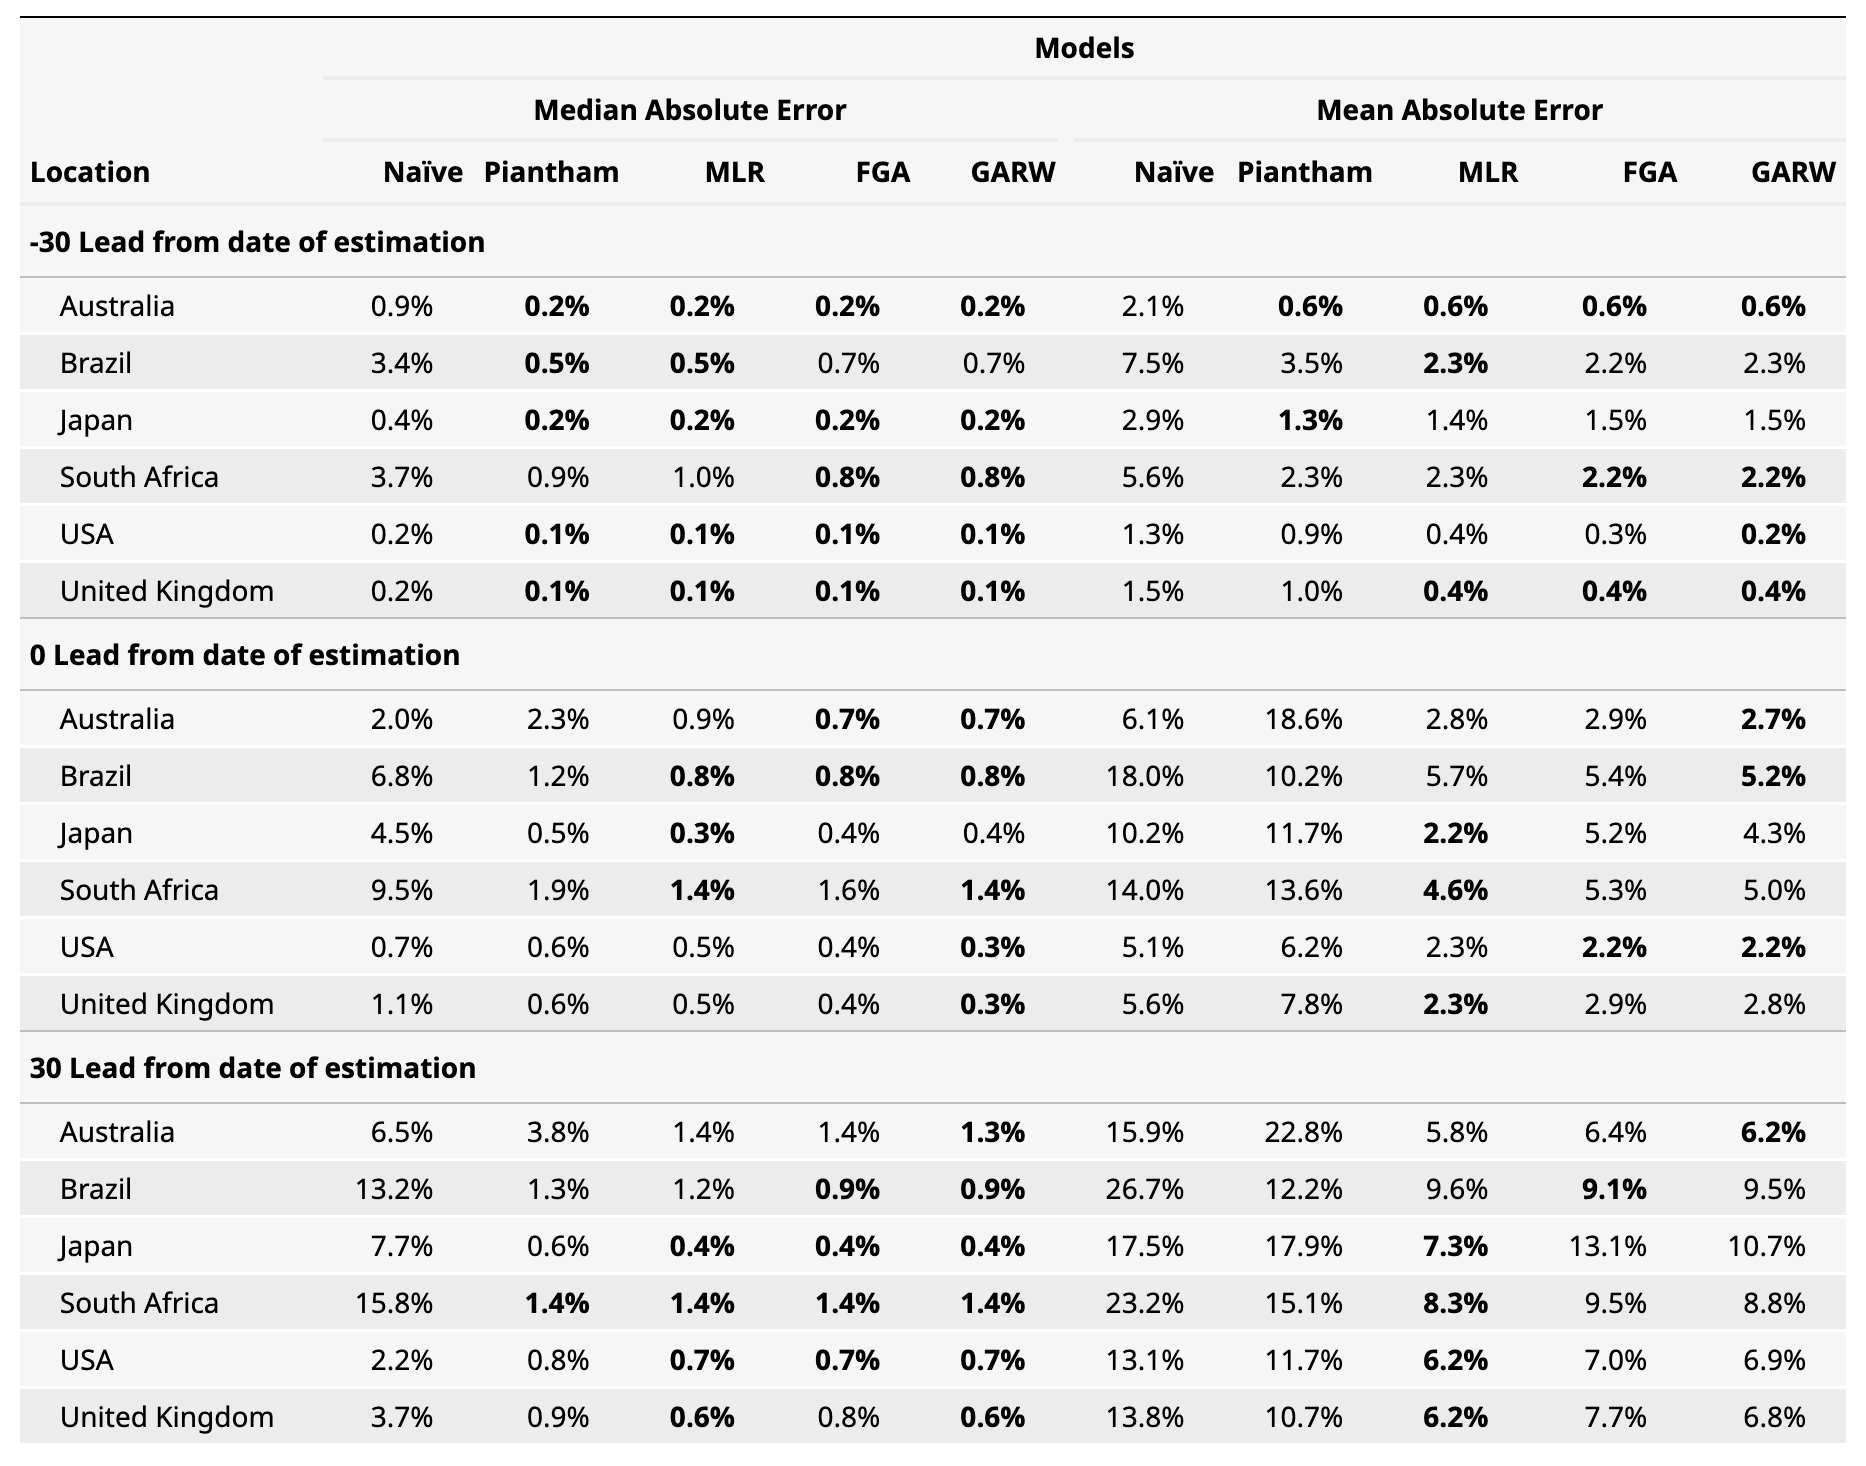
\includegraphics[width=1\textwidth]{figures/model_comp_table.png}
	\caption{
		\textbf{Mean and median absolute error}
		The percentages of median and mean absolute errors at three leads (-30, 0, and +30 days) for each model across 6 countries.
		The values offer a detailed examination of forecast accuracy for these models, highlighting the models with the lowest errors at each forecasting lag, denoted in bold for clarity. 
		}
	
	\label{table:model_comp_table}
\end{table}

Throughout the following discussion, we refer to the `absolute error` (AE) for a given model $m$ and data set $d$ as the difference between the retrospective raw frequencies and the predicted frequencies as:

\begin{equation}
    \mathrm{AE}_{t}^{m,d} = \frac{1}{n} \sum_{v \in V} \left|f_{v}^{d}(t) - \hat{f}^{m,d}_{v}(t) \right|,
\end{equation}

where $f_{v}^{d}(t)$ and $\hat{f}_{v}^{m,d}(t)$ are the retrospective frequencies and the predicted frequencies for model $m$, data  $d$, variant $v$, and time  $t$.

Since we work with data sets that vary both in their location and date of forecast, we often work with the lead time which is defined as the difference between date of observation for the data set and the forecasted date: $l = t - T_{\text{obs}}$.
This enables of us to compare forecasts at different dates within a location.

We compare our predictions to retrospective truth via 7-day smoothed frequency and calculated mean absolute error and median absolute error to assess the relative performance of the models for the six countries (Table~\ref{table:model_comp_table}).
The model with the lowest mean absolute error for each country is highlighted.
As expected we observe decreasing performance across models as lags increase from -30 days, to 0 days to +30 days.
For example, median absolute error increases for the MLR model from 0.1\%--1\% at -30 days to 0.3\%--1.4\% at 0 days, and to 0.4\%--1.4\% at +30 days.
While mean absolute error increases for the MLR model from 0.4\%--2.3\% at -30 days to 2.2\%--5.7\% at 0 days, and to 5.8\%--9.6\% at +30 days.
All four forecasting models perform better than the naive model, with MLR and the variant Rt models FGA and GARW performing slightly better than the Piantham variant Rt model, except for in Australia where MLR, FGA and GARW performed decreased error by 2.4\% median absolute error compared to Piantham.
MLR perform best in +30 lead with lowest mean absolute errors shown in all coutries with the exception of Brazil where FGA performed better by 0.4\%. 
Similar results are apparent when examining median and mean absolute error as a continuous progression from -30 days to +30 days (Fig.~\ref{fig:model_comp_fig}A, ~\ref{fig:model_comp_fig}B ).

Absolute error varies across predictions for individual analysis dates and variants.
Its distribution is heterogeneous with most predictions having very little error, while a subset of predictions have larger error (Fig.~\ref{fig:model_comp_fig}B)
Here we use a 5\% absolute error threshold to classify an acceptable prediction vs unacceptable prediction (shown as dashed line) in both mean and median absolute error calculations.
At +30 days forecast lag we find that the Piantham model has X\%, the MLE model has X\%, the FGA model has X\% and the GARW model has X\% of forecasts with error above this threshold.
This supports previous observation of similar performance across MLR and the FGA and GARW parameterizations of the variant Rt model.



In observing heterogeneity in prediction accuracy, we hypothesized that error is largest for emerging variants when sequence count data is rare.
We investigate this hypothesis by charting how variant-specific growth advantage estimated in the MLR model varied across by analysis date (Fig.~\ref{fig:ga_estimates}).
Generally, we see sharp changes in estimated growth advantage in the first 1-3 weeks when a variant is emerging, but then see less pronounced changes.
Thus it often takes a couple weeks for MLR model to `dial in' estimated growth advantage and accuracy will tend to be poorer in early weeks when variant-specific growth advantage is uncertain.

\begin{figure}[H]
	\centering
    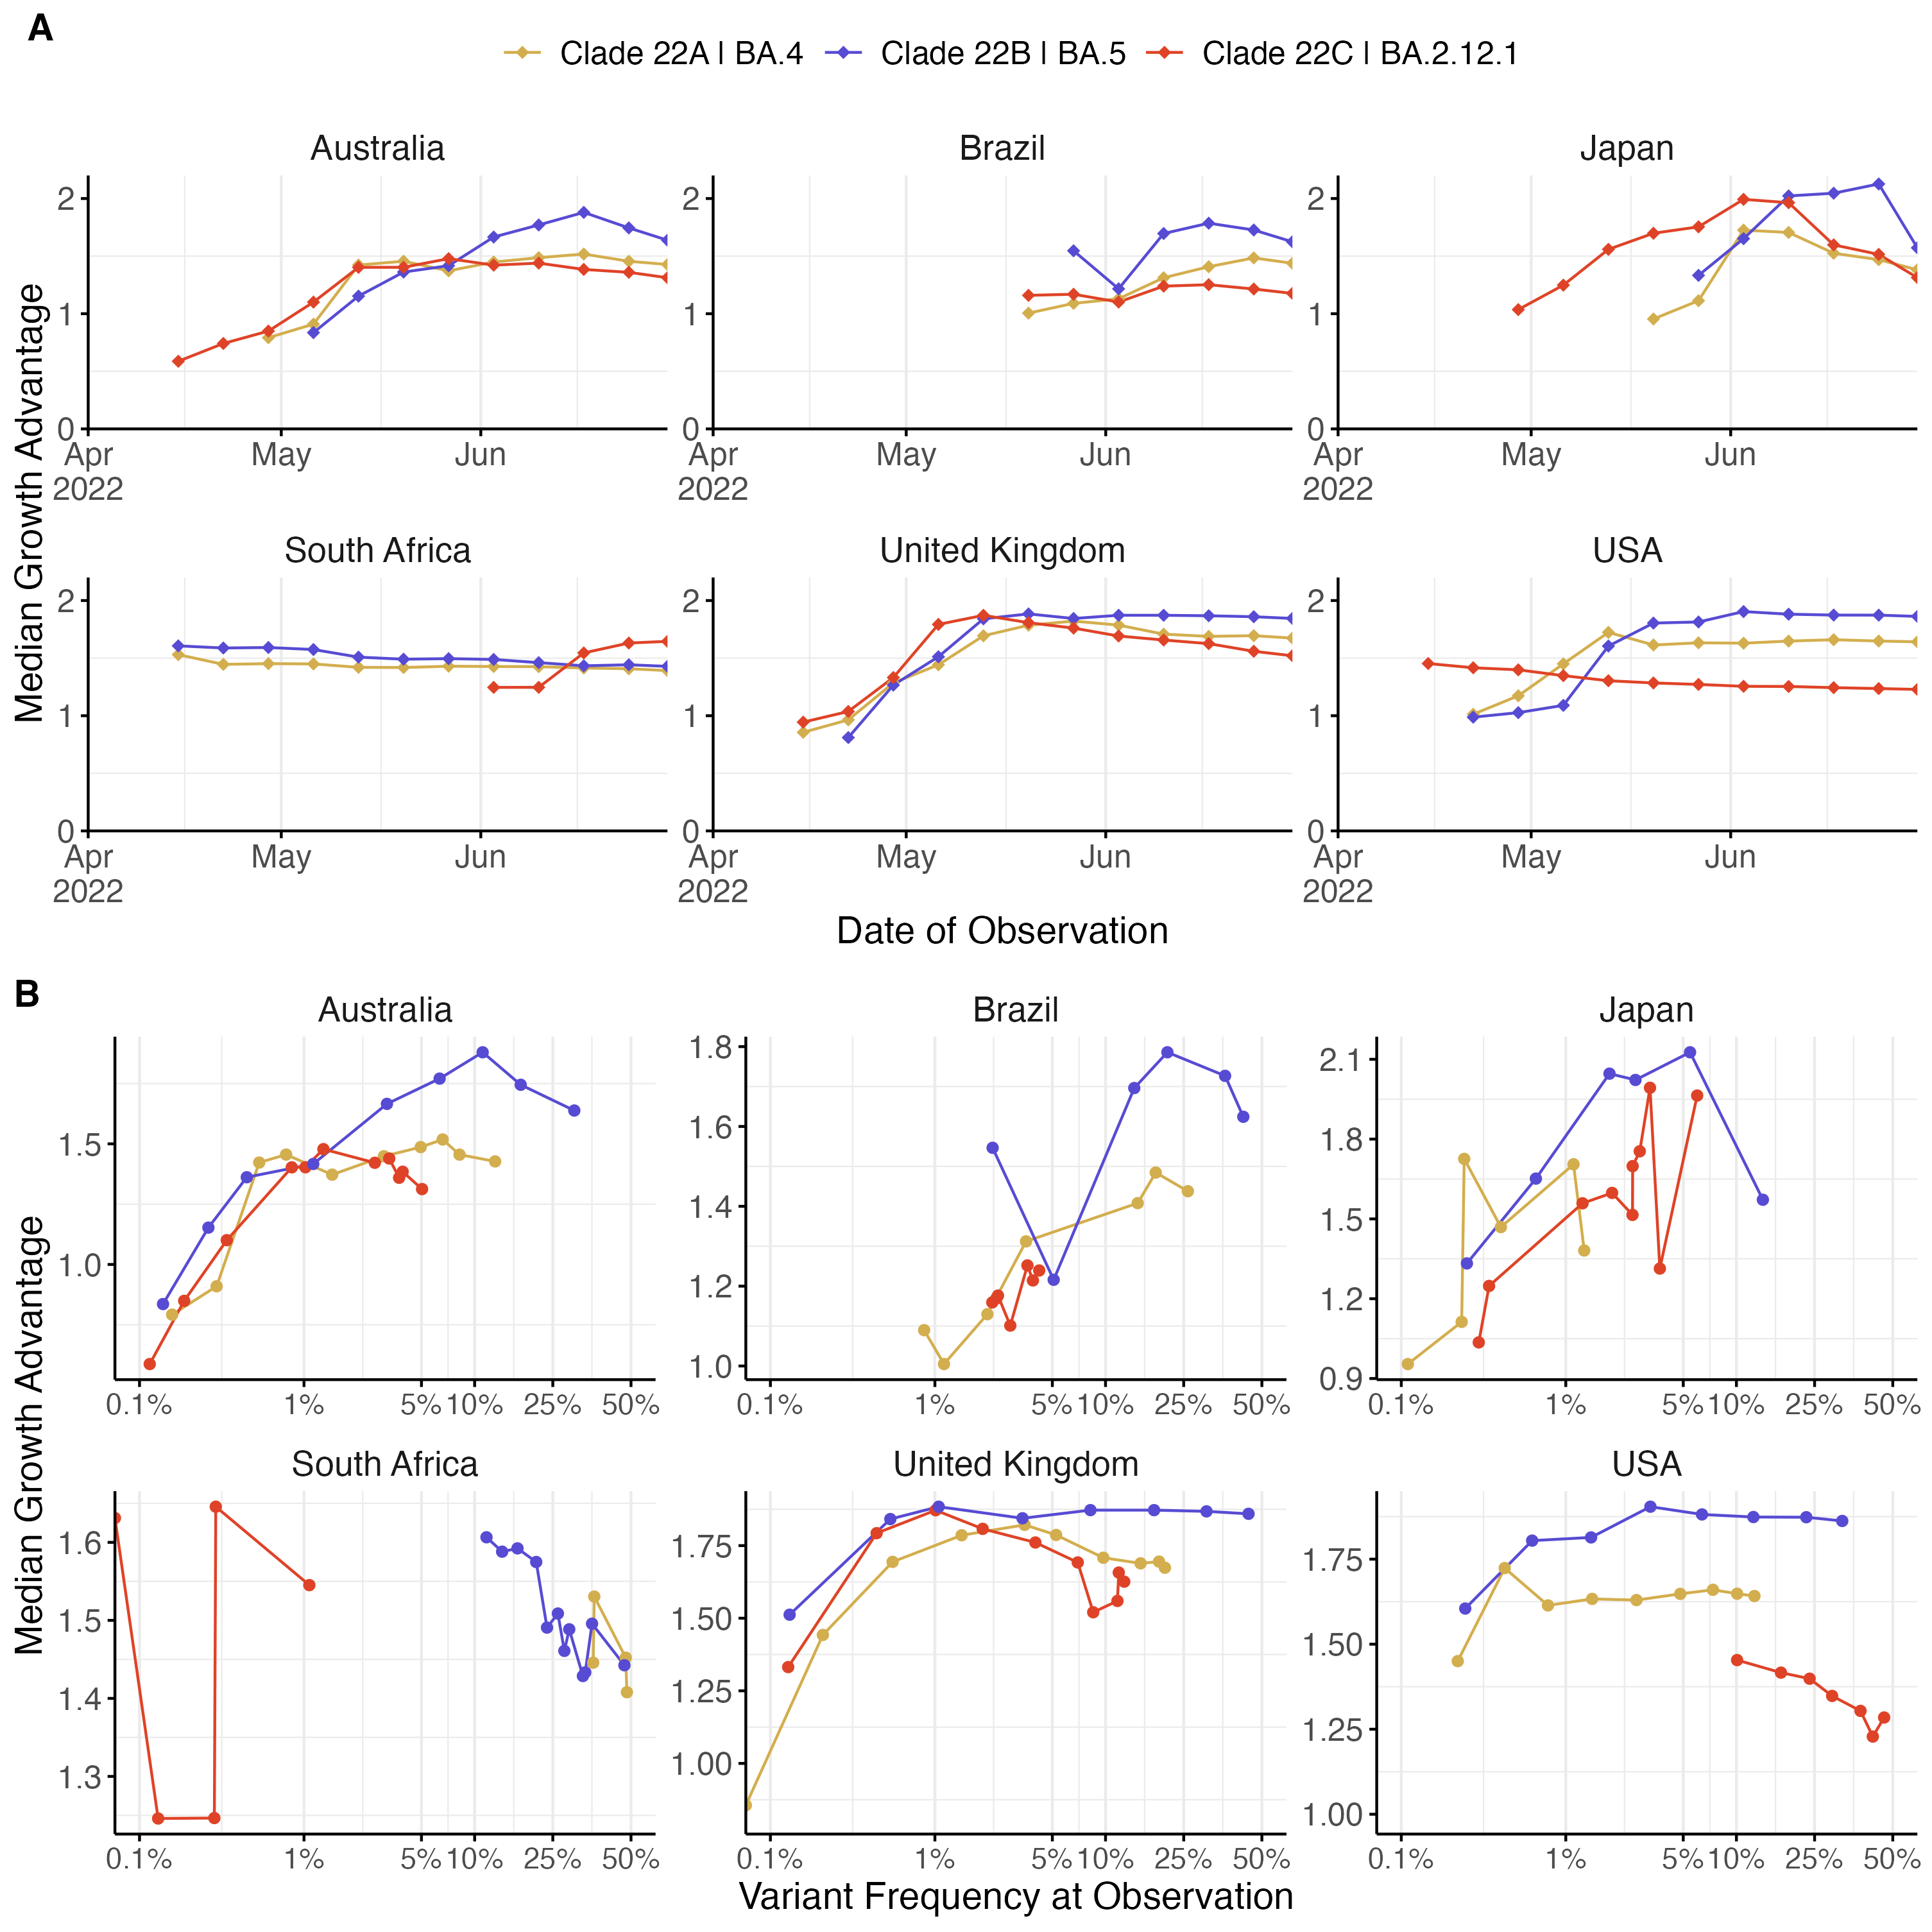
\includegraphics[width=1.0\textwidth]{figures/ga_estimates.png}
	\caption{
		\textbf{Growth advantage of variants varies with analysis date.}
		Growth advantage is estimated via the MLR model and is computed relative to clade 21K (lineage BA.1).
	}
	\label{fig:ga_estimates}
\end{figure}

\subsection*{Genomic surveillance systems and forecast error}

\begin{figure}[tb!]
	\centering
    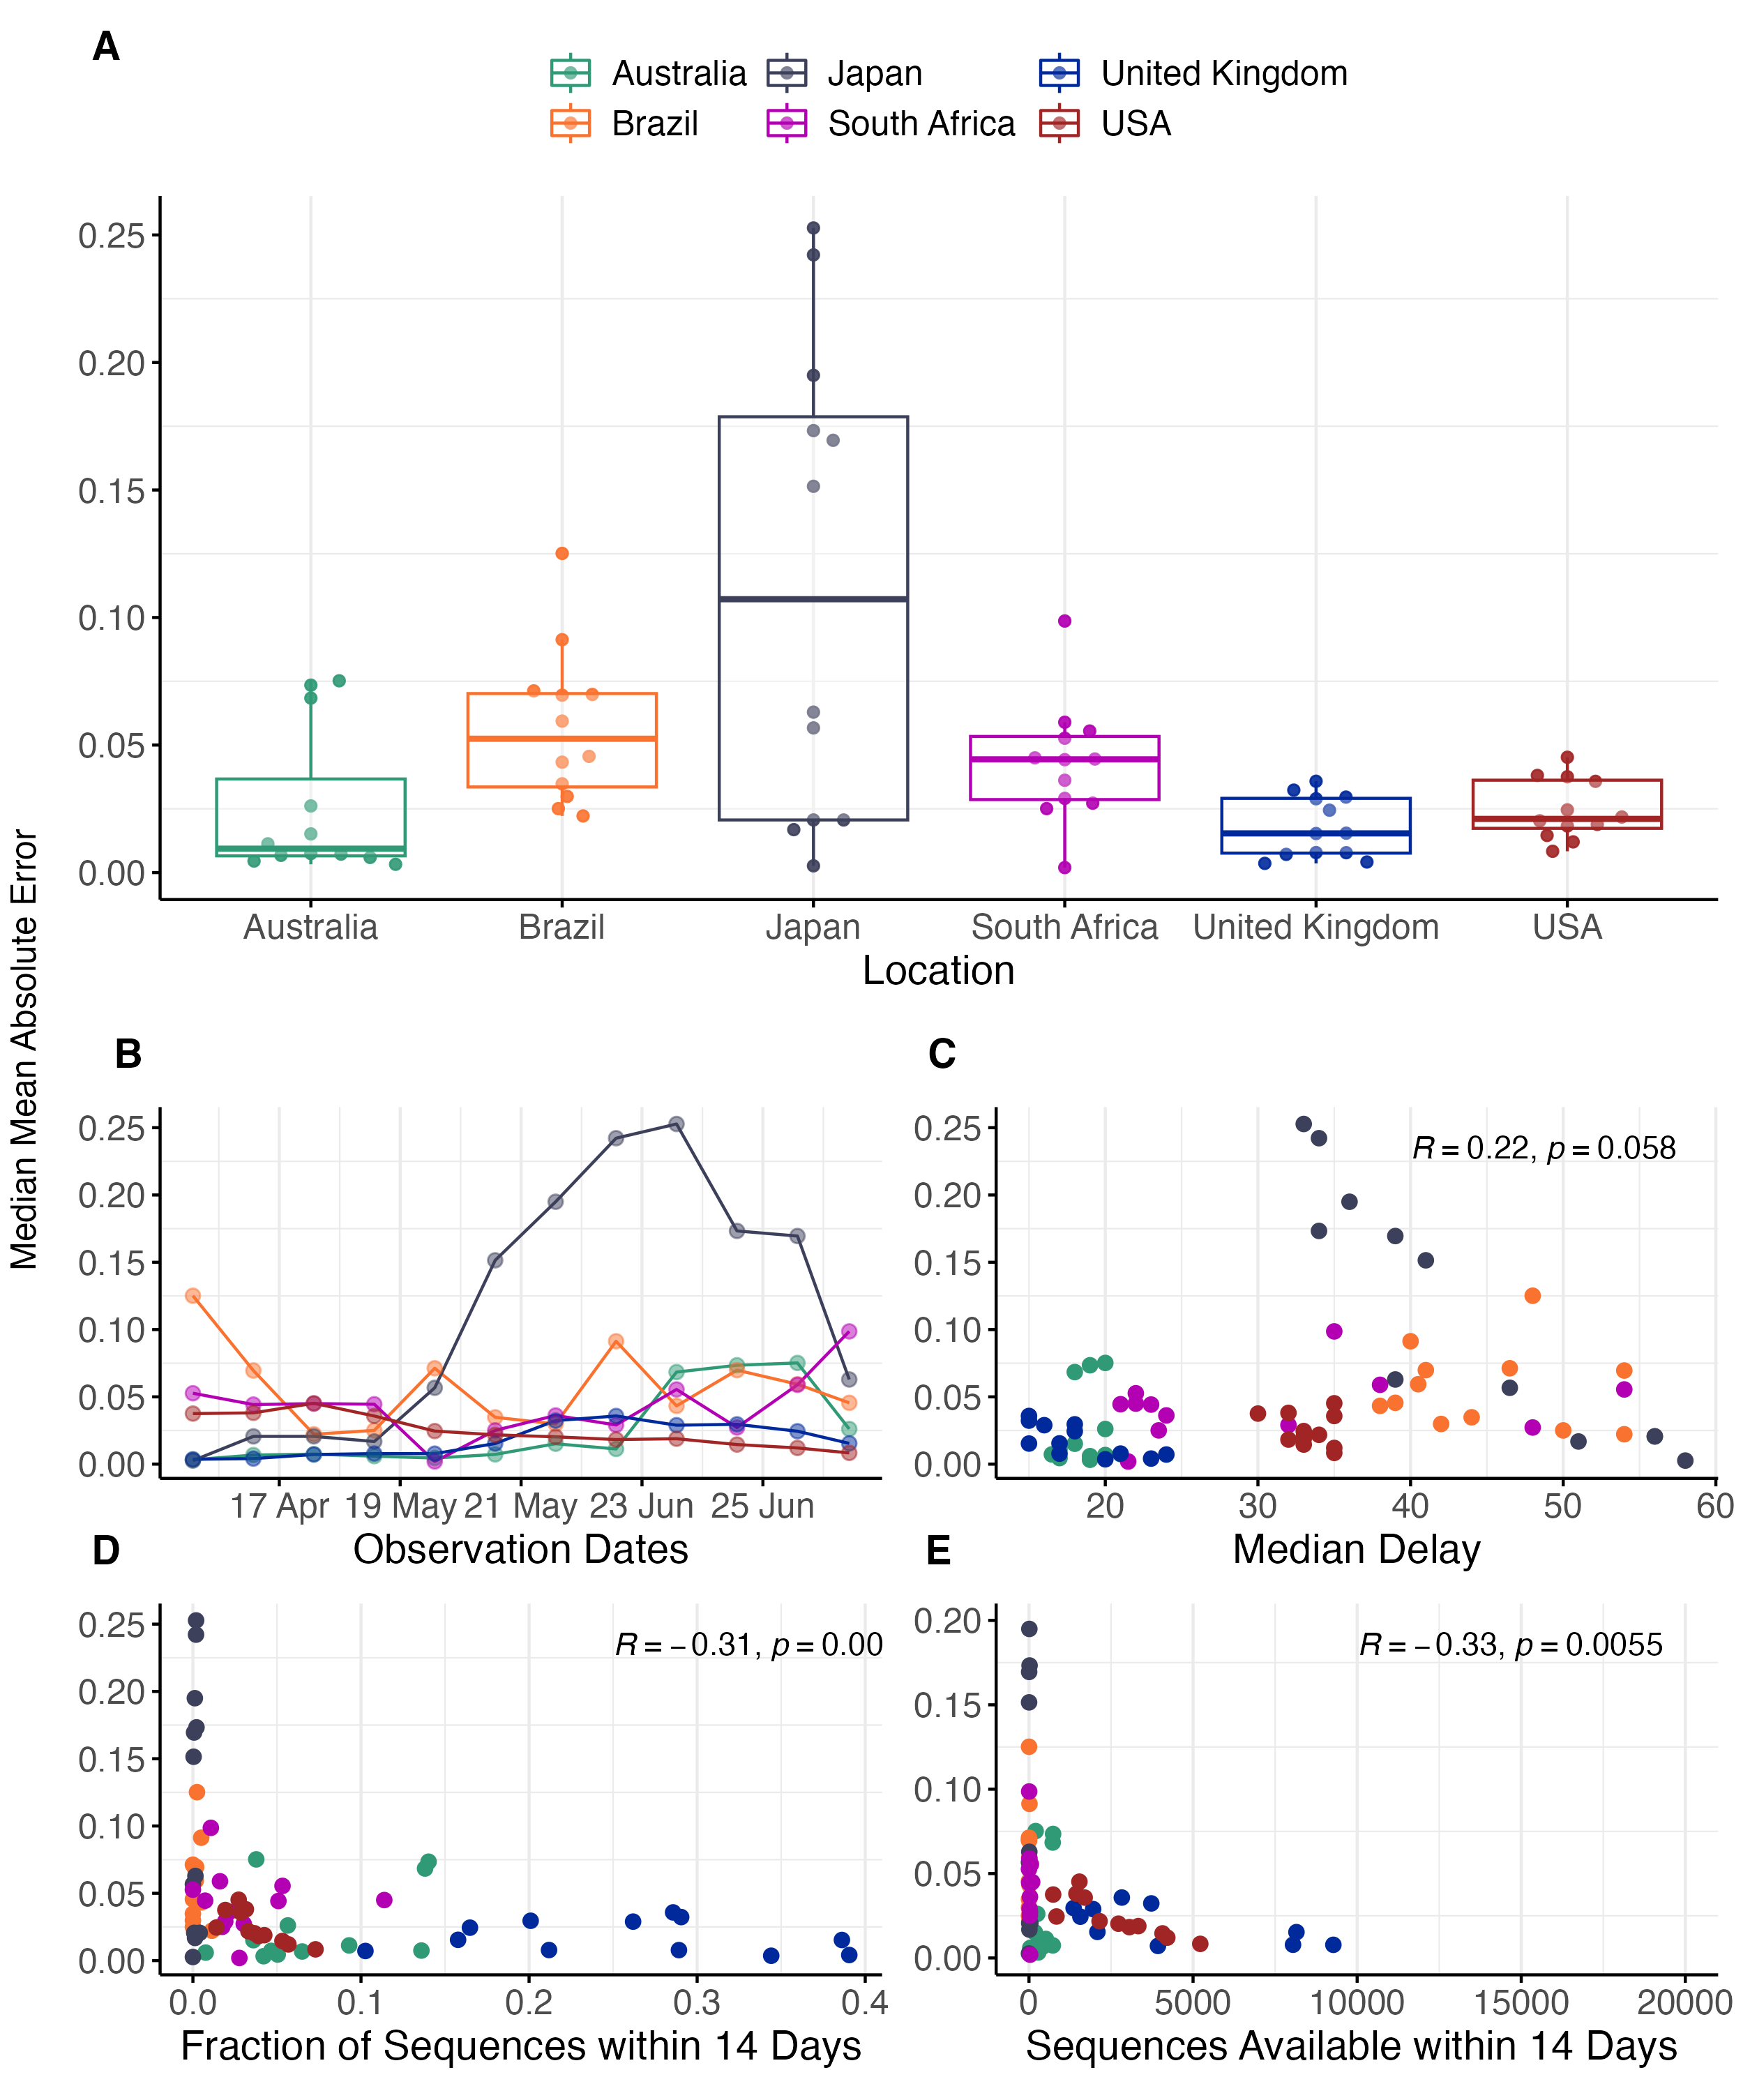
\includegraphics[width=0.85\textwidth]{figures/Var_of_interest.png}
	\caption{
		\textbf{Sequence quantity and quality influence nowcasts error}
    (A) Mean absolute error at nowcast for the MLR model across countries.
		% \tbc{Yes, this was +30 day forecast for the MLR model?}
    \tbc{Points should work exactly like Figure 2B and each point should represent absolute error for a single timepoint and a single variant.}
    \mfc{Points here are as in Figure 2B and represent the mean absolute error at 0 lead time. We take the mean across variants for a single model score. Otherwise, there would be $V$ points stretching vertically for each predictor value.}
		Median and interquartile range of absolute errors are shown as box-and-whisker plots.
		(B-E) Correlation of sequence quality and sequence quantity metrics for given analysis time and country with resulting mean absolute error.
    Correlation strength and significance are calculated via Pearson rank and are inset in each panel.
	}
	\label{fig:vars_of_interest}
\end{figure}

Again, using the MLR model, we find that different countries have consistently different levels of forecasting error with forecasts in Brazil and South Africa showing more error than forecasts in the UK and the USA  (Fig.~\ref{fig:vars_of_interest}A).
We find that broad statistics describing both quantity and quality of sequence data available in at different analysis timepoints and in different genomic surveillance systems correlates with forecasting error (Fig.~\ref{fig:vars_of_interest}B--E).
Using Pearson rank correlations we find that poor sequence quality as measured by proportion of available sequences labeled as `bad' by Nextclade quality control \cite{aksamentov2021nextclade} correlates slightly with mean AE (Fig.~\ref{fig:vars_of_interest}B).
We find that good sequence quantity as measured by total sequences available at analysis has a moderate negative correlation with mean absolute error (Fig.~\ref{fig:vars_of_interest}E).

\begin{figure}[tb!]
    \centering
    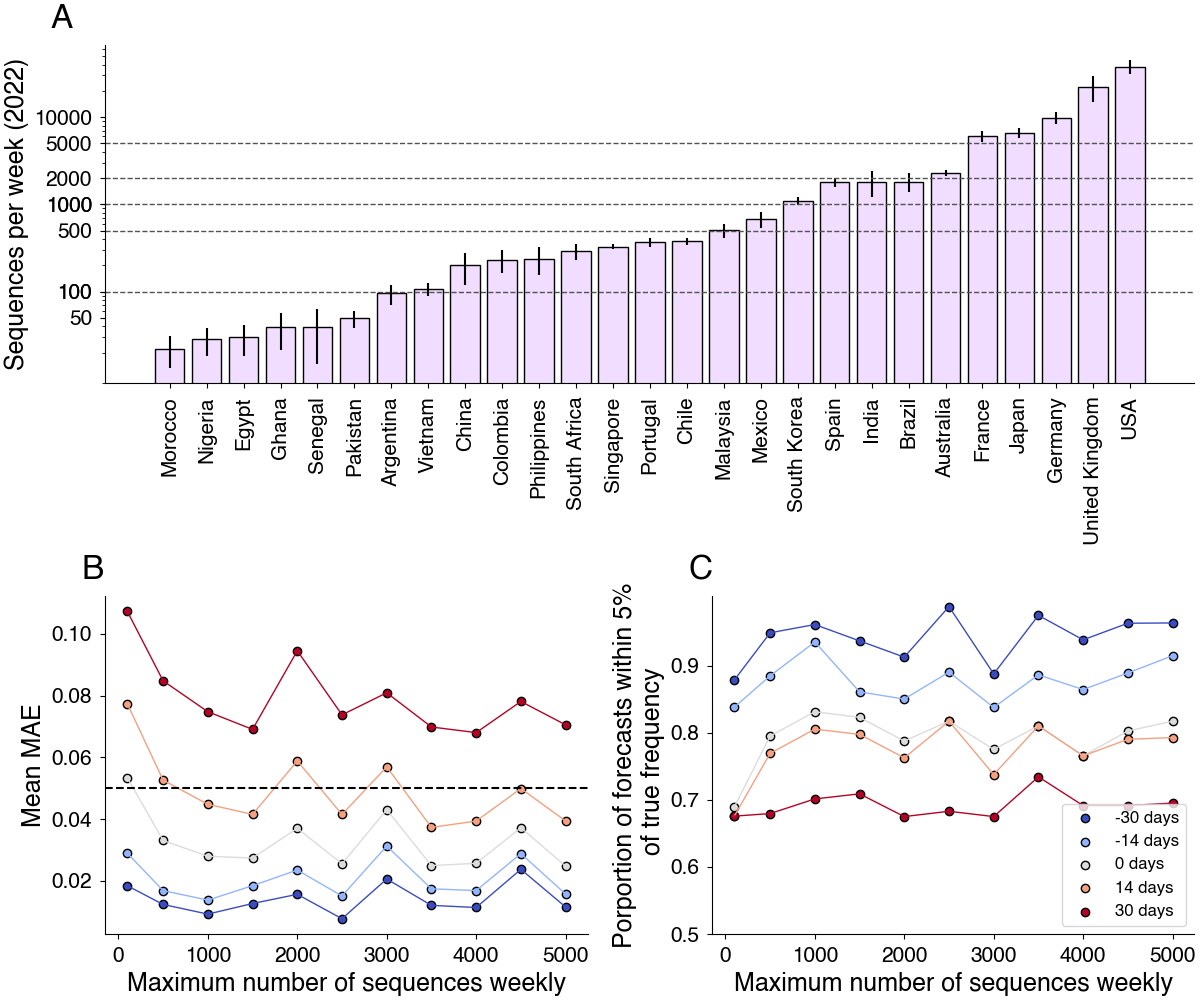
\includegraphics[width=1.0\linewidth]{figures/downscaling_sequencing.png}
    \caption{
			\textbf{Increasing sequencing intensity reduces forecast error}
    	(A) Mean sequences collected per week for selected countries in 2022.
			Intervals are 95\% confidence intervals of the mean.
			Dashed lines correspond to sampling rates used in (B-E).
    	(B, C) Mean absolute error as a function of sequences collected per week colored by forecast horizon (-30 days, -15 days, 0 days, +15 days, +30 days) for the United Kingdom and Denmark.
			The dash line corresponds to 5\% frequency error.
    	(D, E) Proportion of forecasts within 5\% of retrospective frequency as a function of sequences collected for week for the United Kingdom and Denmark.
  	}
    \label{fig:downscaling}
\end{figure}

As suggested by these correlations across countries and time points, we expect that as sequencing intensity decreases, our accuracy in forecasting may vary as we have decreasing levels of resolution in current variant frequencies and estimated growth advantages.
In order to investigate what number of sequences need to collected weekly to keep forecast error within acceptable bounds, we subsampled existing sequences from the United Kingdom and Denmark.
For context, we also computed the mean weekly sequences collected for selected countries globally in 2022 (Fig.~\ref{fig:downscaling}A).
We select the United Kingdom due to its large counts of available sequences, relatively short submission delay, and low forecast error.
We simulate several downscaled data sets by subsampling the collected sequences at multiple thresholds for number of sequences per week and then fit the MLR model to each of the resulting data sets to see how forecast accuracy varies with sampling intensity.
In order to properly account for variability in the subsampled data sets, we generate 5 subsamples per threshold, location, and analysis date.

From this analysis, we find that increasing the number of sequences per week generally decreases the average error, but there are diminishing returns (Fig.~\ref{fig:downscaling}B,D).
Additionally, the effect appears to saturate at different values depending on the forecast length.
We find that for +14 and +30 day forecasts sampling at least 1000 sequences per week is sufficient to minimize forecast error.
In this analysis, we compare the UK to Denmark to explore the difference between paucity of data and stochastic noise due to smaller epidemic size.
However, we arrive at a similar threshold of 1000 sequences per week for both the UK and Denmark  (Fig.~\ref{fig:downscaling}B-E).

%%% DISCUSSION %%%
\section*{Discussion}

% Discussion: Overall model performance and comparison across models (Table 1, Figure 2)
% Discussion: Include distribution of errors (Figure 2B)
% Discussion: Include discussion of MLR vs FGA vs GARW vs Piantham (Table 1, Figure 2)
% Discussion: Include error vs lag (Table 1, Figure 2)

By developing a framework for comparing models of SARS-CoV-2 variant frequency and their forecasts, we find that most models of variant frequency perform well and are able to produce reasonable \jhc{how reasonable?} forecasts.
However, we find that naive models such as a 7-day moving average may not perform well due to the live nature of sequencing efforts e.g. delays between collection and availability of new samples.
Overall, it appears that differences in model accuracy are partially attributable to differences in the surveillance and sequencing efforts.

Consistent with evidence from SARS-CoV-2 time series forecasting analysis \cite{cramer2022unitedforecastinghub}, we find an increase in model errors and their variance as estimates go farther in the future from the observation date.
These long-term forecasts also appear to have heavier tails which indicate increase in extreme values and may be attributable to model break down or the emergence of new variants.

% Discussion: Include discussion of improvement over naive (Table 1, Figure 2)
% Discussion: With specific discussion of improvement over naive model at -30 day hindcast

Our findings suggest that the variations in error patterns observed are likely attributable to the way in which the models handle data issues across different countries.
As such inferences from forecasting models with underlying poor sequencing efforts may not be reliable without a contextual understanding of these limitations.
Additionally, standard modeling practices often involve presenting moving averages of retrospective frequencies of variants as the ``truth''.
However, our analysis of the naive model reveals a substantial discrepancy between the averages of past frequencies and the retrospective truth for all countries, except for the US and UK, where a rigorous sequencing effort is in place.
Importantly, we find that the multinomial logistic regression model (MLR) provides an improvement in accuracy over the naive model for Australia, Brazil, Japan, and South Africa.

% Discussion: We believe the primary source of error is difficulty dealing with the emergence of new variants (Figure 3)

From our analysis of transmission dynamics, we find that it takes a shorter amount of time for different variant clades to stabilize in countries with more robust sequencing efforts.
\jhc{The previous sentence seems to conflate demographics with sequencing capacity.}
Our analysis also suggests that the variability between different countries' growth advantage estimates for different clades may not necessarily be biological but due to data limitations that we show here.
\jhc{What results in the paper support the previous sentence? I don't see where you quantified each country's sequencing capacity and compared that directly to variation in GA.}
We find that at higher frequencies the growth advantage estimates for the clades begin to stabilize though the frequency at which this begins to occur appears to differ by country.

\jhc{Why isn't the following hypothesis the first one to consider instead of sequencing capacity?}
Though our analyses highlight the role of sequencing effort and intensity in reducing forecast error, it is important to note that non-sequencing heterogeneity through the transmission process and pathogen evolution may also explain error.
This could explain why South Africa did not show stabilization in growth advantages due to potentially differing variant dynamics or differences in the sequences effort itself.

% Discussion: Importance of both sequence quantity and sequence quality to forecast accuracy (Figure 4)
% Discussion: Diminishing returns to increasing sequencing capacity (Figure 5)

Analyzing the variation in nowcast and forecast error, we find that overall sequence quality and quantity at time of analysis are associated with nowcast accuracy.
This further supports the idea that high quality sequencing, high intensity sequencing, and quick submission of sequences are useful for providing high accuracy, real-time estimates of variant fitness and frequency.

Subsampling existing data in high sequencing intensity countries, we find that there are diminishing returns to increasing sequencing efforts however maintaining consistent forecasts for variant frequencies can be done with around 1,000 sequences per week.
This level of sequencing enables robust short-term forecasts of pathogen frequency dynamics at the level of a country and highlights the feasibility of pathogen surveillance for evolutionary forecasting.
Though, we are able to see the overall utility of these methods for providing short-term forecasts, we additionally find that no matter how many sequences are obtained some forecast error is maintained with standard methods for frequency forecasts.

% Discussion: We find that short-term forecasts are well supported by simple growth advantage models like MLR
% Discussion: These models fundamentally don't deal with new mutations and thus have limited forecasting horizons
% Discussion: Future modeling work should seek to expand forecasting horizon by incorporating experimental data or otherwise estimating biological impact of future mutations

It is important to point out the limitations of these models. 
While we find simple growth advantage models, such as Multinomial Logistic Regression (MLR), provide robust short-term forecasts, these models do not inherently account for potential mutations and their fitness effects leading to limitations in the effective forecasting horizon. 
To improve future modeling work, we suggest incorporating experimental data to inform fitness change in time including estimating biological impact of future mutations to expand effective forecasting horizon. 

%%% METHODS %%%
\section*{Methods}

\paragraph{Preparing sequence counts and case counts}

We prepared sequence count datasets to replicate a live nowcasting environment using the Nextstrain-curated SARS-CoV-2 sequence metadata which is created using the GISAID database.
For a given observation date, we filtered to all sequences which were collected 90 days before the observation date.
To properly account for submission delays in this collection process, we additionally filtered to those sequences which were submitted before the observation day.
These sequences are then counted according to their Nextstrain clade to produce sequence counts for each clade each day over the period of interest.
These sequence counts are produced independently for 6 countries including Australia, Brazil, Japan, the United States, the United Kingdom, and South Africa.
We repeated this process for a series of observations days which are the 1st and 15th of each month starting with  Janurary 1st, 2022 and ending with December 15th, 2022 giving a total of 24 datasets for each country.
Since two models (FGA and GARW) also use case counts for their estimates, we additionally prepare data sets using case counts over the time periods of interest as available from Our World in Data.

\paragraph{Frequency dynamics and transmission advantages}%

We implemented and evaluated several models of variant frequencies.
Each of these methods estimate variant frequencies over time and as well as estimate the transmission advantage of given variant relative to a baseline variant $R_{t}^{v} / R_{t}^{u}$.

The 4 models of interest are: Multinomial Logistic Regression (MLR), Piantham model \cite{piantham2021estimating}, a fixed growth advantage model (FGA)  \cite{figgins2022sars}, and a growth advantage random walk model (GARW)  \cite{figgins2022sars}.
Details for each of these models can be found in the corresponding citations above.

We provide a brief mathematical overview of these methods below.

The models mentioned above estimate the frequency  $f_{v}(t)$ of variant $v$ at time $t$ using sequence counts and/or case counts of the form described in the previous section.
All models simultaneously estimate the variant transmission advantages $\Delta_{v} = \frac{R_{t}^{v}}{R_{t}^{\text{pivot}}}$ where $R_{t}^{v}$ is the effective reproduction number for variant $v$.
We can interpret these transmission advantages as the relative effective reproduction number of a variant relative to some reference variant.

The multinomial logistic regression model estimates a fixed growth advantage using logistic regression with a variant-specific intercept and time coefficient, so that the frequency of variant $v$ at time $t$ can be modeled as
\begin{align*}
    f_{v}(t) = \frac{\exp(\alpha_{v} + \delta_{v} t)}{\sum_{u} \exp(\alpha_{u} + \delta_{u} t)},
\end{align*}
where $\Delta_{v} = \exp(\delta_{v} \tau)$ for some fixed generation time $\tau$.
The Piantham model relies on an approximation to the renewal equation wherein new infections do not vary greatly over the generation time of the virus.
This model generalizes the MLR in that it accounts for non-fixed generation time though it assumes little overall case growth. \cite{piantham2021estimating}

The fixed growth advantage model uses a renewal equation model based on both case counts and sequence counts, but assumes that the growth advantage $\Delta_{v}$ is constant in time. \cite{figgins2022sars}
The growth advantage random walk model also uses a renewal equation model based on both case counts and sequences, but allows variant growth advantages to vary smoothly in time. \cite{figgins2022sars}

The models used all differ in the complexity of their assumptions in computing the variant growth advantage which may affect forecasting accuracy.
Growth advantages presented in this manuscript are estimated relative to the baseline Omicron 21L (BA.1) strain, providing a point of reference for competing growth advantages and how median values change over time.
Further details on the model formats can be found in their respective citations.
All models were implemented using the evofr (evolutionary forecasting) software package in Python (https://pypi.org/project/evofr/) using Numpyro for inference.

We compare the four models to a naive model which is implemented as a 7-day moving average on the retrospective raw frequencies.

\paragraph{Evaluation Criteria}

We evaluate the error between the model predicted frequencies and the truth set averaged across each variant at a given time point using the mean absolute error and median absolute error.
%should MAE equation be moved here?
\paragraph{Generating predictors of error}

We explored four key variables to describe the effect of sequencing efforts on nowcast errors and estimated Pearson correlations with the mean absolute nowcast errors.
These variables are defined as proportion of bad quality control (QC) sequences, fraction of sequences available within 14 days of the prediction time, total sequences availability within 14 days of the prediction time, median delay of sequence submission (Figure~\ref{fig:vars_of_interest} B-E).
To calculate these variables, we selected a 14-day window of data before each and every observation date and used the collection and submission dates to determine their availability.
Total sequence availability was calculated by dividing the sequences where submission date was before the date of analysis by the total collected sequencies and similarily fraction of sequences at observation was estimated. 
Sequence submission delay was calculated by taking the difference between the submission date and the date of collection.
Bad QC sequence proportion was estimated by dividing the sequences with bad Nextstrain classification by the total collected sequences.  
All estimates were run for all defined dates of analyses across all countries. 
All variables were calculated using Rstudio statistical software \cite{Rstudio2022}


%TODO: Add details on how we generate points for \ref{fig:vars_of_interest}


\paragraph{Downscaling historical sequencing effort}

We explored the effects of scaling back sequencing efforts to assess the effect of sequencing volume on nowcast and forecast errors.
Using the sequencing data from the United Kingdom and Denmark, we subsampled existing available sequences at the time of analysis at a rate of 100, 200, 400, 600, 800, 1000, 1200, 1400, 1600, 1800, and 2000 sequences per week for the same observation dates and study period used in the previous analyses, generating 5 subsampled data sets for each sequencing rate, location, and analysis date.
We then fit the MLR forecast model to each resulting data set and forecast up to 30 days after observation date and compared these forecasts to the truth set in previous sections to compute the forecast error for each model.
To better understand how the forecast error varies with sequencing intensity and forecast length, we computed the fraction of forecasts within an error tolerance (5\% AE) as well as the average error at different sequence threshold and lag times.


\section*{Data and code accessibility}

Sequence data including date and location of collection as well as clade annotation was obtained via the Nextstrain-curated
dataset that pulls data from GISAID database. 
A full list of sequences analyzed with accession numbers, derived data of sequence counts and case counts, along with all source code used to analyze
this data and produce figures is available via the GitHub repository https://github.com/blab/ncov-forecasting-fit

%%% REFERENCES %%%
\bibliographystyle{plos}
\bibliography{ncov-forecasting-fit.bib}

\end{document}
